% -*- root: ../../DAT2-A423_Project_Report.tex -*-
\section{LSB implementation}
\label{sec:lsb-implementation}
During the beginning of the project, to learn more and understand how this algorithm works, as well as see first-hand what social media sites re-encoded images, we created a small prototype of a programme, which is able to conceal an image within another image, using the LSB algorithm. 

By storing the information we want concealed in the two least significant bits, we can keep all of the original information, and changing each pixel of the cover image, by a maximum value of 3 or $00000011_2$, the concealed image will almost be invisible to the naked eye.

To do this, we had to make some restrictions on how big the cover image had to be relatively to the to-be-concealed image. 
To not cause corruption and to ensure all information got saved, the cover image has to be four times as big as the hidden image, more specifically twice its height, and twice its width. 
Each pixel of the concealed image will be stored within four pixels of the cover image, each masked differently, hence the cover image has to be four times its size. 
We do this to get as much of the concealed image's information stored within the cover as possible.

To make both images easier to work with, we store each pixel's colour in their own array of type \lstinline|Color|.
To store each pixel within the cover, we first mask the cover to remove the information stored within the least significant bits using the bitwise operator \&. 
We then mask the concealed image to only keep the information stored in two bits, then right-shift those bits so the result, will be a byte where only the least-significant-bits, can be 1, and then, add this information to the cover. 
The result will be a slightly changed pixel by a value between 0 and 3 for the Red, Green and Blue channels. 
The first pixel in the cover will contain the two most significant bits of the concealed image, the next will contain the third and fourth, and so on. 
To get back the image information, we once again use the bitwise \& operator, to only keep the information within the least-significant bits of every pixel, then left-shift them accordingly and save this to a Colour array. Once every pixel has been read, the Colour array can be transformed into an image which looks just like the original.

The result of concealing \ref{img2}, within \ref{img1}, can be seen in \ref{img3}

\begin{figure}[]
	\centering
	\begin{subfigure}[b]{.3\linewidth}
		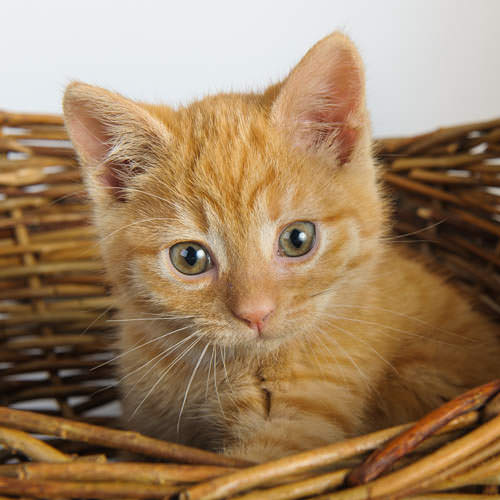
\includegraphics[width=\linewidth]{cover.jpg}
		\captionof{figure}{Cover image}
		\label{img1}
	\end{subfigure}
	\hspace{.02\linewidth}
	\begin{subfigure}[b]{.3\linewidth}
		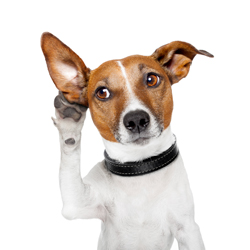
\includegraphics[width=\linewidth]{message.jpg}
		\captionof{figure}{Message image}
		\label{img2}
	\end{subfigure}
	\hspace{.02\linewidth}

	\begin{subfigure}[b]{.4\linewidth}
		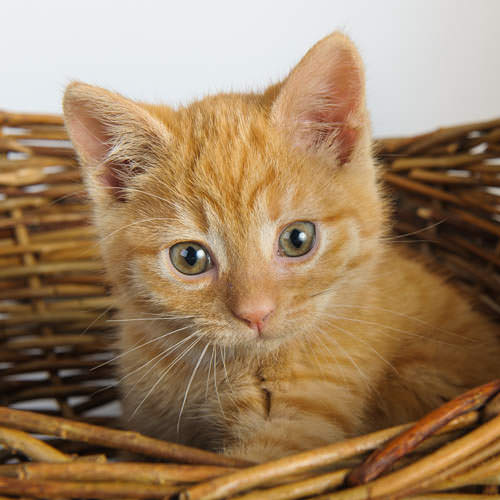
\includegraphics[width=.97\textwidth]{stego.jpg}
		\captionof{figure}{Steganographic image}
		\label{img3}
	\end{subfigure}
	\caption{The steganographic process}\label{LSBDemo}
\end{figure} 


% -*- root: ../../DAT2-A423_Project_Report.tex -*-
\begin{algorithm}
\caption{LSB}
\label{alg1}
\begin{algorithmic}
\REQUIRE True-color images $v = \{v^0,v^1,v^2\ldots v^{NM}\}$ with size $M \times N$ and $c  = \{c^0,c^1,c^2\ldots c^{(NM)/2}\}$ where $c^{xN/2+y}$ is the pixel at location $(x,y)$
\ENSURE True-color image $h  = \{h^0,h^1,h^2\ldots h^{NM}\}$ of size $M \times N$ and where $h^{xN+y}$ is the pixel at location $(x,y)$ and where $c$ is embedded in $v$

\STATE{$k := 1$}
\FOR {$i:=1$ \TO $i=N/2$}
	\FOR {$j:=1$ \TO $j=4$}
		\STATE{Set the first 6 bits in the R, G and B bytes $k$th element of $h$ to be the first 6 bits of the R, G and B bytes of the $k$th element of $v$}

		\STATE{Set the 7th bit in the R, G and B bytes in the $k$th element of $h$ with the $(j\cdot 2 - 1)$th bit in the R, G and B bytes in the $i$th element in $c$}

		\STATE{Set the 8th bit in the R, G and B bytes in the $k$th element of $h$ with the $(j\cdot 2)$th bit in the R, G and B bytes in the $i$th element in $c$}
		
		\STATE{$k := k + 1$}
	\ENDFOR
\ENDFOR

\RETURN $h$
\end{algorithmic}
\end{algorithm}